\documentclass[a4paper]{IEEEtran}

\usepackage{graphicx}

\title{Cloud Computing: \\ Report}
\author{Steffan Norberhuis\\ 1509306 \and
 Rogier Slag\\ 1507761}

\author{
    \IEEEauthorblockN{Steffan Norberhuis, Rogier Slag}\\
    \IEEEauthorblockA{1509306, 1507761}
}

\begin{document}
\maketitle
\begin{center}
\today
\end{center}

\section{Abstract}


\section{Introduction}
%Recommended size abstract and introduction 1 page
%Describe the problem

%Related work

%To be implemented system

%structure of arcticle

\section{Background on Application}
%1-3 paragraph
%Describe application

%Requirements


\section{System Design}
%Recommended Size 1.5 pages

\subsection{Resource Management Architecture}
%Design

%Inter operation provisioning

%Allocation

%Reliability

%Monitoring components


\subsection{System Policies}


\section{Experimental Results}
%Recommended size 1.5 pages
In this section we will describe the experimental setup and the experiments themselves.
Observations and experiments are also included in this section.

\subsection{Experimental setup}
%Describe working environments
The system was developed for Amazon AWS and was tested on that platform.
Amazon AWS provides different types of instances and we used \emph{t2.micro} instances.
Our workload is mostly CPU intensive.
These are the smallest instances provided and we could achieve higher performance on larger instances,
 but they were chosen because they are Free Tier eligible.
Amazon describes these instances as CPU's operating at 2.5GHz and having 1 GB of memory.

%Describe general workload
We created a workload generator that generates an artificial workload.
The workload generator creates a new task at a regular interval and offers this task to the system using the input bucket.
The task can either be a completely new task or with a certain chance be a task already offered to the system before.
The tasks consist of encoding a movie from one format to another format.

%Describe monitoring tools and libraries
To monitor the system we used \emph{The Simple Logging Facade for Java} (SLF4J) in combination with \emph{Log4J}.
SLF4J provides a facade for Log4J to allow other logging backends to be configured at runtime.
We used simple logging output to measure the performance and other statistics of the system.
%other tools

\subsection{Experiments}
%Desribe the experiments per system feature
%Format: describe workload, present operation, analyze result.
\subsubsection{Automation}
We performed no specific experiments to test the automation of our system.
But the other experiments have shown that we have achieved a very high level of automation.
To start we only have to do a minimal amount of mandatory steps and after that the system runs fully without manual intervention.
The first step is to create a EC2 instance that will act as a master instance.
After that we upload the code and run an install script that sets up the master instance.
The last step is to build the code and run it.

\subsubsection{Provisioning}
%Provisioning time
In our first experiment we wanted to see how long it takes to provision a worker node and how long it takes before it is fully ready to service tasks.
Our experiment consists of the provisioner provisioning continiously a single worker after the previous worker becomes fully ready.
The experiment showed that the average and median time of provisioning a fully working node is 2 minutes and 31 seconds.
The minimum time of provisioning was 2 minutes and the maximum 4 minutes and 47 seconds.
A note has to be made that the timing is done with a granularity of 15 seconds, because that was the interval we checked if nodes came online.
But this experiment still gives a very good indication of the time it takes to provision a worker node.

The second experiment we conducted is to have the workload generator generate 100 jobs with a random interval between 10 and 30 seconds.
The experiment is to test that our provisioner provisions more nodes and terminates these nodes after the 100 jobs are completed.
At first the system builds a backlog of queues and the provisioner conservatively allocates more workers.
After 27 minutes all jobs are finished and it can be seen that the provisioner quickly terminates the unnecessary workers.
In this downscaling it is now conservative.
At the end a tail can be seen where one worker is kept running.
This data is plotted in Fig. \ref{fig:100-workers} and Fig. \ref{fig:100-tasks}.

\begin{figure}[ht]
	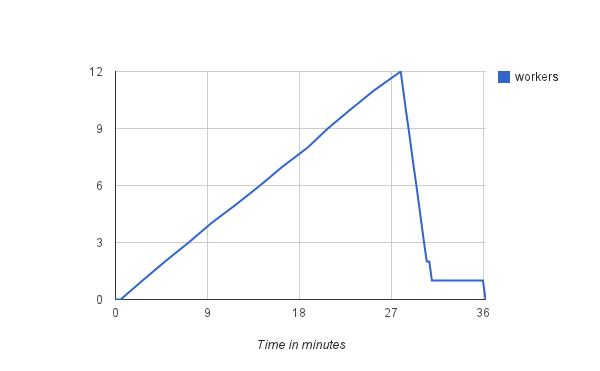
\includegraphics[scale=0.5]{fig/100workers.png}
	\label{fig:100-workers}
	\caption{Amount of workers}
\end{figure}

\begin{figure}[ht]
	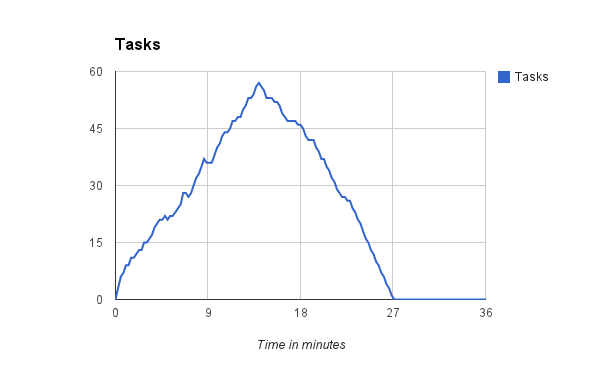
\includegraphics[scale=0.5]{fig/100tasks.png}
	\label{fig:100-tasks}
	\caption{Amount of queued tasks}
\end{figure}

\subsubsection{Allocation}
One experiment we run 

\subsubsection{Reliability}

\subsubsection{Monitoring components}

%Report charged-time
%Report charged cost
%Report service metrics

\section{Discussion}

\section{Conclusion}

\appendix
\section{Time Sheets}
\end{document}
